\documentclass[border=10pt]{standalone}
\usepackage{tikz}
\begin{document}
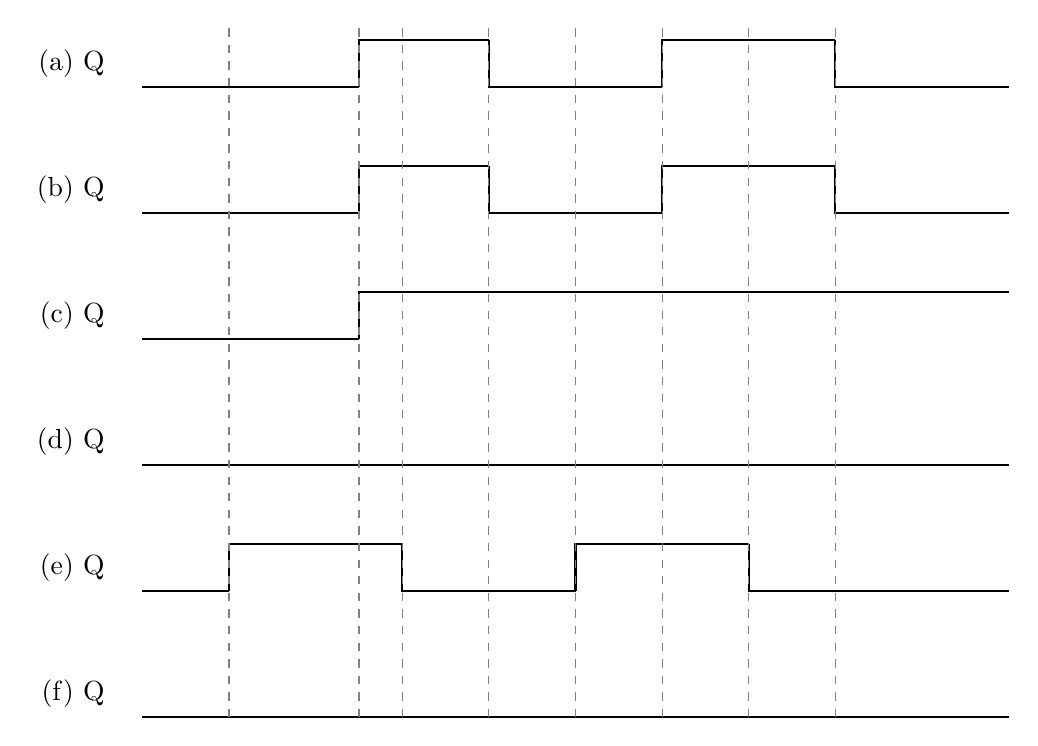
\begin{tikzpicture}[x=1cm, y=1cm, font=\normalsize, line width=0.8pt]
  % 图 8.06 六子图 Q 答案波形（对应课程站 10-26 页 8.6「完整解答」逐段结论）：
  % 横轴 0–100% 等分 20 格，每格 0.55 cm，总宽 11.0 cm；高电平 0.6 cm。
  % 百分比 -> 格：10->2, 25->5, 30->6, 40->8, 50->10, 60->12, 70->14, 80->16。
  % 竖虚线在 10/25/30/40/50/60/70/80% 八处，贯穿六行（x、行距为全图坐标，
  % 放在最后一个 scope 外层画）。
  % 各行电平段（格）：
  %   (a) (b) 五段 0–5 | 5–8 | 8–12 | 12–16 | 16–20 = 0,1,0,1,0
  %   (c) 恒 1； (d) (f) 恒 0；
  %   (e) 0–2 | 2–6 | 6–10 | 10–14 | 14–20 = 0,1,0,1,0（10/30/50/70% 翻转）。
  \def\seg{0.55}
  \def\hi{0.6}
  \def\total{11.0}

  % (a) Q：0 0-25% | 1 25-40% | 0 40-60% | 1 60-80% | 0 80-100%
  \begin{scope}[yshift=0cm]
    \node[anchor=east] at (-0.35,\hi/2) {(a) Q};
    \draw (0,0) -- (5*\seg,0);
    \draw (5*\seg,0) -- (5*\seg,\hi) -- (8*\seg,\hi);
    \draw (8*\seg,\hi) -- (8*\seg,0) -- (12*\seg,0);
    \draw (12*\seg,0) -- (12*\seg,\hi) -- (16*\seg,\hi);
    \draw (16*\seg,\hi) -- (16*\seg,0) -- (\total,0);
  \end{scope}

  % (b) Q：与 (a) 相同
  \begin{scope}[yshift=-1.6cm]
    \node[anchor=east] at (-0.35,\hi/2) {(b) Q};
    \draw (0,0) -- (5*\seg,0);
    \draw (5*\seg,0) -- (5*\seg,\hi) -- (8*\seg,\hi);
    \draw (8*\seg,\hi) -- (8*\seg,0) -- (12*\seg,0);
    \draw (12*\seg,0) -- (12*\seg,\hi) -- (16*\seg,\hi);
    \draw (16*\seg,\hi) -- (16*\seg,0) -- (\total,0);
  \end{scope}

  % (c) Q：0-25% 低、25% 起恒 1（页面 10-26 作业第 118 行）
  \begin{scope}[yshift=-3.2cm]
    \node[anchor=east] at (-0.35,\hi/2) {(c) Q};
    \draw (0,0) -- (5*\seg,0);
    \draw (5*\seg,0) -- (5*\seg,\hi) -- (\total,\hi);
  \end{scope}

  % (d) Q：恒 0
  \begin{scope}[yshift=-4.8cm]
    \node[anchor=east] at (-0.35,\hi/2) {(d) Q};
    \draw (0,0) -- (\total,0);
  \end{scope}

  % (e) Q：0 0-10% | 1 10-30% | 0 30-50% | 1 50-70% | 0 70-100%
  \begin{scope}[yshift=-6.4cm]
    \node[anchor=east] at (-0.35,\hi/2) {(e) Q};
    \draw (0,0) -- (2*\seg,0);
    \draw (2*\seg,0) -- (2*\seg,\hi) -- (6*\seg,\hi);
    \draw (6*\seg,\hi) -- (6*\seg,0) -- (10*\seg,0);
    \draw (10*\seg,0) -- (10*\seg,\hi) -- (14*\seg,\hi);
    \draw (14*\seg,\hi) -- (14*\seg,0) -- (\total,0);
  \end{scope}

  % (f) Q：恒 0
  \begin{scope}[yshift=-8.0cm]
    \node[anchor=east] at (-0.35,\hi/2) {(f) Q};
    \draw (0,0) -- (\total,0);
  \end{scope}

  % 八条竖虚线（10/25/30/40/50/60/70/80%），贯穿六行
  \foreach \gx in {2,5,6,8,10,12,14,16}{
    \draw[dashed, line width=0.4pt, gray] (\gx*\seg,\hi+0.15) -- (\gx*\seg,-8.0);
  }
\end{tikzpicture}
\end{document}
